\documentclass[twoside]{book}

% Packages required by doxygen
\usepackage{fixltx2e}
\usepackage{calc}
\usepackage{doxygen}
\usepackage[export]{adjustbox} % also loads graphicx
\usepackage{graphicx}
\usepackage[utf8]{inputenc}
\usepackage{makeidx}
\usepackage{multicol}
\usepackage{multirow}
\PassOptionsToPackage{warn}{textcomp}
\usepackage{textcomp}
\usepackage[nointegrals]{wasysym}
\usepackage[table]{xcolor}

% Font selection
\usepackage[T1]{fontenc}
\usepackage[scaled=.90]{helvet}
\usepackage{courier}
\usepackage{amssymb}
\usepackage{sectsty}
\renewcommand{\familydefault}{\sfdefault}
\allsectionsfont{%
  \fontseries{bc}\selectfont%
  \color{darkgray}%
}
\renewcommand{\DoxyLabelFont}{%
  \fontseries{bc}\selectfont%
  \color{darkgray}%
}
\newcommand{\+}{\discretionary{\mbox{\scriptsize$\hookleftarrow$}}{}{}}

% Page & text layout
\usepackage{geometry}
\geometry{%
  a4paper,%
  top=2.5cm,%
  bottom=2.5cm,%
  left=2.5cm,%
  right=2.5cm%
}
\tolerance=750
\hfuzz=15pt
\hbadness=750
\setlength{\emergencystretch}{15pt}
\setlength{\parindent}{0cm}
\setlength{\parskip}{3ex plus 2ex minus 2ex}
\makeatletter
\renewcommand{\paragraph}{%
  \@startsection{paragraph}{4}{0ex}{-1.0ex}{1.0ex}{%
    \normalfont\normalsize\bfseries\SS@parafont%
  }%
}
\renewcommand{\subparagraph}{%
  \@startsection{subparagraph}{5}{0ex}{-1.0ex}{1.0ex}{%
    \normalfont\normalsize\bfseries\SS@subparafont%
  }%
}
\makeatother

% Headers & footers
\usepackage{fancyhdr}
\pagestyle{fancyplain}
\fancyhead[LE]{\fancyplain{}{\bfseries\thepage}}
\fancyhead[CE]{\fancyplain{}{}}
\fancyhead[RE]{\fancyplain{}{\bfseries\leftmark}}
\fancyhead[LO]{\fancyplain{}{\bfseries\rightmark}}
\fancyhead[CO]{\fancyplain{}{}}
\fancyhead[RO]{\fancyplain{}{\bfseries\thepage}}
\fancyfoot[LE]{\fancyplain{}{}}
\fancyfoot[CE]{\fancyplain{}{}}
\fancyfoot[RE]{\fancyplain{}{\bfseries\scriptsize Generated by Doxygen }}
\fancyfoot[LO]{\fancyplain{}{\bfseries\scriptsize Generated by Doxygen }}
\fancyfoot[CO]{\fancyplain{}{}}
\fancyfoot[RO]{\fancyplain{}{}}
\renewcommand{\footrulewidth}{0.4pt}
\renewcommand{\chaptermark}[1]{%
  \markboth{#1}{}%
}
\renewcommand{\sectionmark}[1]{%
  \markright{\thesection\ #1}%
}

% Indices & bibliography
\usepackage{natbib}
\usepackage[titles]{tocloft}
\setcounter{tocdepth}{3}
\setcounter{secnumdepth}{5}
\makeindex

% Hyperlinks (required, but should be loaded last)
\usepackage{ifpdf}
\ifpdf
  \usepackage[pdftex,pagebackref=true]{hyperref}
\else
  \usepackage[ps2pdf,pagebackref=true]{hyperref}
\fi
\hypersetup{%
  colorlinks=true,%
  linkcolor=blue,%
  citecolor=blue,%
  unicode%
}

% Custom commands
\newcommand{\clearemptydoublepage}{%
  \newpage{\pagestyle{empty}\cleardoublepage}%
}

\usepackage{caption}
\captionsetup{labelsep=space,justification=centering,font={bf},singlelinecheck=off,skip=4pt,position=top}

%===== C O N T E N T S =====

\begin{document}

% Titlepage & ToC
\hypersetup{pageanchor=false,
             bookmarksnumbered=true,
             pdfencoding=unicode
            }
\pagenumbering{alph}
\begin{titlepage}
\vspace*{7cm}
\begin{center}%
{\Large My Project }\\
\vspace*{1cm}
{\large Generated by Doxygen 1.8.14}\\
\end{center}
\end{titlepage}
\clearemptydoublepage
\pagenumbering{roman}
\tableofcontents
\clearemptydoublepage
\pagenumbering{arabic}
\hypersetup{pageanchor=true}

%--- Begin generated contents ---
\chapter{Symulation}
\label{md__r_e_a_d_m_e}
\Hypertarget{md__r_e_a_d_m_e}
\input{md__r_e_a_d_m_e}
\chapter{Namespace Index}
\section{Namespace List}
Here is a list of all namespaces with brief descriptions\+:\begin{DoxyCompactList}
\item\contentsline{section}{\mbox{\hyperlink{namespacesample}{sample}} }{\pageref{namespacesample}}{}
\end{DoxyCompactList}

\chapter{Hierarchical Index}
\section{Class Hierarchy}
This inheritance list is sorted roughly, but not completely, alphabetically\+:\begin{DoxyCompactList}
\item \contentsline{section}{sample.\+Alert}{\pageref{classsample_1_1_alert}}{}
\item \contentsline{section}{sample.\+Controller}{\pageref{classsample_1_1_controller}}{}
\item Runnable\begin{DoxyCompactList}
\item \contentsline{section}{sample.\+Color\+Square}{\pageref{classsample_1_1_color_square}}{}
\end{DoxyCompactList}
\item Application\begin{DoxyCompactList}
\item \contentsline{section}{sample.\+Main}{\pageref{classsample_1_1_main}}{}
\end{DoxyCompactList}
\item Rectangle\begin{DoxyCompactList}
\item \contentsline{section}{sample.\+Color\+Square}{\pageref{classsample_1_1_color_square}}{}
\end{DoxyCompactList}
\end{DoxyCompactList}

\chapter{Class Index}
\section{Class List}
Here are the classes, structs, unions and interfaces with brief descriptions\+:\begin{DoxyCompactList}
\item\contentsline{section}{\mbox{\hyperlink{classsample_1_1_alert}{sample.\+Alert}} }{\pageref{classsample_1_1_alert}}{}
\item\contentsline{section}{\mbox{\hyperlink{classsample_1_1_color_square}{sample.\+Color\+Square}} }{\pageref{classsample_1_1_color_square}}{}
\item\contentsline{section}{\mbox{\hyperlink{classsample_1_1_controller}{sample.\+Controller}} }{\pageref{classsample_1_1_controller}}{}
\item\contentsline{section}{\mbox{\hyperlink{classsample_1_1_main}{sample.\+Main}} }{\pageref{classsample_1_1_main}}{}
\end{DoxyCompactList}

\chapter{File Index}
\section{File List}
Here is a list of all files with brief descriptions\+:\begin{DoxyCompactList}
\item\contentsline{section}{src/sample/\mbox{\hyperlink{_alert_8java}{Alert.\+java}} }{\pageref{_alert_8java}}{}
\item\contentsline{section}{src/sample/\mbox{\hyperlink{_color_square_8java}{Color\+Square.\+java}} }{\pageref{_color_square_8java}}{}
\item\contentsline{section}{src/sample/\mbox{\hyperlink{_controller_8java}{Controller.\+java}} }{\pageref{_controller_8java}}{}
\item\contentsline{section}{src/sample/\mbox{\hyperlink{_main_8java}{Main.\+java}} }{\pageref{_main_8java}}{}
\end{DoxyCompactList}

\chapter{Namespace Documentation}
\hypertarget{namespacesample}{}\section{Package sample}
\label{namespacesample}\index{sample@{sample}}
\subsection*{Classes}
\begin{DoxyCompactItemize}
\item 
class \mbox{\hyperlink{classsample_1_1_alert}{Alert}}
\item 
class \mbox{\hyperlink{classsample_1_1_color_square}{Color\+Square}}
\item 
class \mbox{\hyperlink{classsample_1_1_controller}{Controller}}
\item 
class \mbox{\hyperlink{classsample_1_1_main}{Main}}
\end{DoxyCompactItemize}

\chapter{Class Documentation}
\hypertarget{classsample_1_1_alert}{}\section{sample.\+Alert Class Reference}
\label{classsample_1_1_alert}\index{sample.\+Alert@{sample.\+Alert}}
\subsection*{Static Public Member Functions}
\begin{DoxyCompactItemize}
\item 
static void \mbox{\hyperlink{classsample_1_1_alert_a56b2f1e797e0f5f4fff8493b91ab33c4}{display}} (String title, String message)
\end{DoxyCompactItemize}


\subsection{Member Function Documentation}
\mbox{\Hypertarget{classsample_1_1_alert_a56b2f1e797e0f5f4fff8493b91ab33c4}\label{classsample_1_1_alert_a56b2f1e797e0f5f4fff8493b91ab33c4}} 
\index{sample\+::\+Alert@{sample\+::\+Alert}!display@{display}}
\index{display@{display}!sample\+::\+Alert@{sample\+::\+Alert}}
\subsubsection{\texorpdfstring{display()}{display()}}
{\footnotesize\ttfamily static void sample.\+Alert.\+display (\begin{DoxyParamCaption}\item[{String}]{title,  }\item[{String}]{message }\end{DoxyParamCaption})\hspace{0.3cm}{\ttfamily [inline]}, {\ttfamily [static]}}

Method for displaying error messages.


\begin{DoxyParams}{Parameters}
{\em title} & Name of the handled \mbox{\hyperlink{}{Exception}}. \\
\hline
{\em message} & \mbox{\hyperlink{}{Exception\#get\+Message()}} of handled \mbox{\hyperlink{}{Exception}}. \\
\hline
\end{DoxyParams}


The documentation for this class was generated from the following file\+:\begin{DoxyCompactItemize}
\item 
src/sample/\mbox{\hyperlink{_alert_8java}{Alert.\+java}}\end{DoxyCompactItemize}

\hypertarget{classsample_1_1_color_square}{}\section{sample.\+Color\+Square Class Reference}
\label{classsample_1_1_color_square}\index{sample.\+Color\+Square@{sample.\+Color\+Square}}
Inheritance diagram for sample.\+Color\+Square\+:\begin{figure}[H]
\begin{center}
\leavevmode
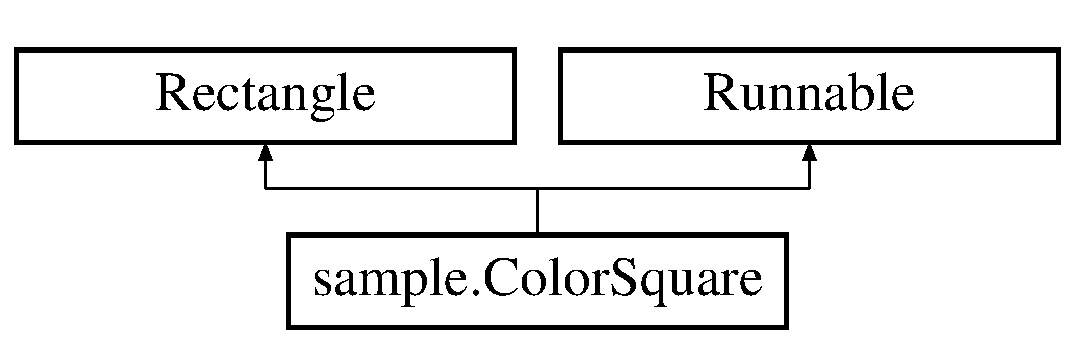
\includegraphics[height=2.000000cm]{classsample_1_1_color_square}
\end{center}
\end{figure}
\subsection*{Public Member Functions}
\begin{DoxyCompactItemize}
\item 
synchronized void \mbox{\hyperlink{classsample_1_1_color_square_a01bfc80ce93985adcaf9f26226a5166c}{run}} ()
\end{DoxyCompactItemize}
\subsection*{Package Functions}
\begin{DoxyCompactItemize}
\item 
\mbox{\hyperlink{classsample_1_1_color_square_a2273dc7c774e92a81ce858facc815ec7}{Color\+Square}} (double \mbox{\hyperlink{classsample_1_1_color_square_af4e8f71262ff634ecd5d6261853b023d}{probability}}, long \mbox{\hyperlink{classsample_1_1_color_square_ac96754f907bed6644d7a18e5992af853}{delay}}, double size, Random \mbox{\hyperlink{classsample_1_1_color_square_a398146a0cc15168fc6fbe5aac3e9f50b}{random}})  throws Illegal\+Argument\+Exception 
\item 
void \mbox{\hyperlink{classsample_1_1_color_square_a3089d9adec502bdcbec959c142872397}{kill}} ()
\item 
void \mbox{\hyperlink{classsample_1_1_color_square_a8bc5e469f5dc2dd0a9a1963112b77fee}{set\+Neighbours}} (\mbox{\hyperlink{classsample_1_1_color_square}{Color\+Square}}\mbox{[}$\,$\mbox{]} \mbox{\hyperlink{classsample_1_1_color_square_a262acfde2a2981d945f37c9600904ff1}{neighbours}})
\item 
void \mbox{\hyperlink{classsample_1_1_color_square_ac913da0d2207fc676be2892fd9a9f5be}{consider\+Eight\+Neighbours}} ()
\item 
void \mbox{\hyperlink{classsample_1_1_color_square_ac487f0d013c9da85fbfbb5c5221eb1e5}{consider\+Four\+Neightbours}} ()
\item 
void \mbox{\hyperlink{classsample_1_1_color_square_a7a9627028e034d129f9d408c89226aab}{explode}} ()
\item 
void \mbox{\hyperlink{classsample_1_1_color_square_a268fbcc6abfcd0a2f74d94f067a9c2c7}{set\+Random\+Color}} ()
\end{DoxyCompactItemize}
\subsection*{Private Member Functions}
\begin{DoxyCompactItemize}
\item 
void \mbox{\hyperlink{classsample_1_1_color_square_a47856df2afb0e0dcdf11dfe5801570c9}{set\+Average\+Neighbours\+Color}} ()
\end{DoxyCompactItemize}
\subsection*{Private Attributes}
\begin{DoxyCompactItemize}
\item 
double \mbox{\hyperlink{classsample_1_1_color_square_af4e8f71262ff634ecd5d6261853b023d}{probability}}
\item 
long \mbox{\hyperlink{classsample_1_1_color_square_ac96754f907bed6644d7a18e5992af853}{delay}}
\item 
Random \mbox{\hyperlink{classsample_1_1_color_square_a398146a0cc15168fc6fbe5aac3e9f50b}{random}}
\item 
\mbox{\hyperlink{classsample_1_1_color_square}{Color\+Square}} \mbox{[}$\,$\mbox{]} \mbox{\hyperlink{classsample_1_1_color_square_a262acfde2a2981d945f37c9600904ff1}{neighbours}}
\item 
boolean \mbox{\hyperlink{classsample_1_1_color_square_ac89c88958f422f4b2293215274f1d958}{alive}}
\item 
int \mbox{\hyperlink{classsample_1_1_color_square_aa261ae0dcf7928c1b8f6ac86ecb3f1de}{considered\+Neighbours}} = 4
\end{DoxyCompactItemize}


\subsection{Constructor \& Destructor Documentation}
\mbox{\Hypertarget{classsample_1_1_color_square_a2273dc7c774e92a81ce858facc815ec7}\label{classsample_1_1_color_square_a2273dc7c774e92a81ce858facc815ec7}} 
\index{sample\+::\+Color\+Square@{sample\+::\+Color\+Square}!Color\+Square@{Color\+Square}}
\index{Color\+Square@{Color\+Square}!sample\+::\+Color\+Square@{sample\+::\+Color\+Square}}
\subsubsection{\texorpdfstring{Color\+Square()}{ColorSquare()}}
{\footnotesize\ttfamily sample.\+Color\+Square.\+Color\+Square (\begin{DoxyParamCaption}\item[{double}]{probability,  }\item[{long}]{delay,  }\item[{double}]{size,  }\item[{Random}]{random }\end{DoxyParamCaption}) throws Illegal\+Argument\+Exception\hspace{0.3cm}{\ttfamily [inline]}, {\ttfamily [package]}}

Constructor for \mbox{\hyperlink{classsample_1_1_color_square}{Color\+Square}}.


\begin{DoxyParams}{Parameters}
{\em probability} & Probability of \mbox{\hyperlink{classsample_1_1_color_square_a268fbcc6abfcd0a2f74d94f067a9c2c7}{set\+Random\+Color()}}. \\
\hline
{\em delay} & Delay of \mbox{\hyperlink{classsample_1_1_color_square_a01bfc80ce93985adcaf9f26226a5166c}{run()}}. \\
\hline
{\em size} & Size of a \mbox{\hyperlink{classsample_1_1_color_square}{Color\+Square}} object. \\
\hline
{\em random} & \mbox{\hyperlink{}{Random}} object for generaating random values.\\
\hline
\end{DoxyParams}

\begin{DoxyExceptions}{Exceptions}
{\em Illegal\+Argument\+Exception} & if parameters are invalid. \\
\hline
\end{DoxyExceptions}


\subsection{Member Function Documentation}
\mbox{\Hypertarget{classsample_1_1_color_square_ac913da0d2207fc676be2892fd9a9f5be}\label{classsample_1_1_color_square_ac913da0d2207fc676be2892fd9a9f5be}} 
\index{sample\+::\+Color\+Square@{sample\+::\+Color\+Square}!consider\+Eight\+Neighbours@{consider\+Eight\+Neighbours}}
\index{consider\+Eight\+Neighbours@{consider\+Eight\+Neighbours}!sample\+::\+Color\+Square@{sample\+::\+Color\+Square}}
\subsubsection{\texorpdfstring{consider\+Eight\+Neighbours()}{considerEightNeighbours()}}
{\footnotesize\ttfamily void sample.\+Color\+Square.\+consider\+Eight\+Neighbours (\begin{DoxyParamCaption}{ }\end{DoxyParamCaption})\hspace{0.3cm}{\ttfamily [inline]}, {\ttfamily [package]}}

\mbox{\Hypertarget{classsample_1_1_color_square_ac487f0d013c9da85fbfbb5c5221eb1e5}\label{classsample_1_1_color_square_ac487f0d013c9da85fbfbb5c5221eb1e5}} 
\index{sample\+::\+Color\+Square@{sample\+::\+Color\+Square}!consider\+Four\+Neightbours@{consider\+Four\+Neightbours}}
\index{consider\+Four\+Neightbours@{consider\+Four\+Neightbours}!sample\+::\+Color\+Square@{sample\+::\+Color\+Square}}
\subsubsection{\texorpdfstring{consider\+Four\+Neightbours()}{considerFourNeightbours()}}
{\footnotesize\ttfamily void sample.\+Color\+Square.\+consider\+Four\+Neightbours (\begin{DoxyParamCaption}{ }\end{DoxyParamCaption})\hspace{0.3cm}{\ttfamily [inline]}, {\ttfamily [package]}}

\mbox{\Hypertarget{classsample_1_1_color_square_a7a9627028e034d129f9d408c89226aab}\label{classsample_1_1_color_square_a7a9627028e034d129f9d408c89226aab}} 
\index{sample\+::\+Color\+Square@{sample\+::\+Color\+Square}!explode@{explode}}
\index{explode@{explode}!sample\+::\+Color\+Square@{sample\+::\+Color\+Square}}
\subsubsection{\texorpdfstring{explode()}{explode()}}
{\footnotesize\ttfamily void sample.\+Color\+Square.\+explode (\begin{DoxyParamCaption}{ }\end{DoxyParamCaption})\hspace{0.3cm}{\ttfamily [inline]}, {\ttfamily [package]}}

\mbox{\Hypertarget{classsample_1_1_color_square_a3089d9adec502bdcbec959c142872397}\label{classsample_1_1_color_square_a3089d9adec502bdcbec959c142872397}} 
\index{sample\+::\+Color\+Square@{sample\+::\+Color\+Square}!kill@{kill}}
\index{kill@{kill}!sample\+::\+Color\+Square@{sample\+::\+Color\+Square}}
\subsubsection{\texorpdfstring{kill()}{kill()}}
{\footnotesize\ttfamily void sample.\+Color\+Square.\+kill (\begin{DoxyParamCaption}{ }\end{DoxyParamCaption})\hspace{0.3cm}{\ttfamily [inline]}, {\ttfamily [package]}}

Method kills \mbox{\hyperlink{classsample_1_1_color_square}{Color\+Square}} object by setting \mbox{\hyperlink{classsample_1_1_color_square_ac89c88958f422f4b2293215274f1d958}{alive}} to false. \mbox{\Hypertarget{classsample_1_1_color_square_a01bfc80ce93985adcaf9f26226a5166c}\label{classsample_1_1_color_square_a01bfc80ce93985adcaf9f26226a5166c}} 
\index{sample\+::\+Color\+Square@{sample\+::\+Color\+Square}!run@{run}}
\index{run@{run}!sample\+::\+Color\+Square@{sample\+::\+Color\+Square}}
\subsubsection{\texorpdfstring{run()}{run()}}
{\footnotesize\ttfamily synchronized void sample.\+Color\+Square.\+run (\begin{DoxyParamCaption}{ }\end{DoxyParamCaption})\hspace{0.3cm}{\ttfamily [inline]}}

\mbox{\Hypertarget{classsample_1_1_color_square_a47856df2afb0e0dcdf11dfe5801570c9}\label{classsample_1_1_color_square_a47856df2afb0e0dcdf11dfe5801570c9}} 
\index{sample\+::\+Color\+Square@{sample\+::\+Color\+Square}!set\+Average\+Neighbours\+Color@{set\+Average\+Neighbours\+Color}}
\index{set\+Average\+Neighbours\+Color@{set\+Average\+Neighbours\+Color}!sample\+::\+Color\+Square@{sample\+::\+Color\+Square}}
\subsubsection{\texorpdfstring{set\+Average\+Neighbours\+Color()}{setAverageNeighboursColor()}}
{\footnotesize\ttfamily void sample.\+Color\+Square.\+set\+Average\+Neighbours\+Color (\begin{DoxyParamCaption}{ }\end{DoxyParamCaption})\hspace{0.3cm}{\ttfamily [inline]}, {\ttfamily [private]}}

Method sets color of this to average of neighbours. \mbox{\Hypertarget{classsample_1_1_color_square_a8bc5e469f5dc2dd0a9a1963112b77fee}\label{classsample_1_1_color_square_a8bc5e469f5dc2dd0a9a1963112b77fee}} 
\index{sample\+::\+Color\+Square@{sample\+::\+Color\+Square}!set\+Neighbours@{set\+Neighbours}}
\index{set\+Neighbours@{set\+Neighbours}!sample\+::\+Color\+Square@{sample\+::\+Color\+Square}}
\subsubsection{\texorpdfstring{set\+Neighbours()}{setNeighbours()}}
{\footnotesize\ttfamily void sample.\+Color\+Square.\+set\+Neighbours (\begin{DoxyParamCaption}\item[{\mbox{\hyperlink{classsample_1_1_color_square}{Color\+Square}} \mbox{[}$\,$\mbox{]}}]{neighbours }\end{DoxyParamCaption})\hspace{0.3cm}{\ttfamily [inline]}, {\ttfamily [package]}}

Method sets \mbox{\hyperlink{classsample_1_1_color_square_a262acfde2a2981d945f37c9600904ff1}{neighbours}}.


\begin{DoxyParams}{Parameters}
{\em neighbours} & \\
\hline
\end{DoxyParams}
\mbox{\Hypertarget{classsample_1_1_color_square_a268fbcc6abfcd0a2f74d94f067a9c2c7}\label{classsample_1_1_color_square_a268fbcc6abfcd0a2f74d94f067a9c2c7}} 
\index{sample\+::\+Color\+Square@{sample\+::\+Color\+Square}!set\+Random\+Color@{set\+Random\+Color}}
\index{set\+Random\+Color@{set\+Random\+Color}!sample\+::\+Color\+Square@{sample\+::\+Color\+Square}}
\subsubsection{\texorpdfstring{set\+Random\+Color()}{setRandomColor()}}
{\footnotesize\ttfamily void sample.\+Color\+Square.\+set\+Random\+Color (\begin{DoxyParamCaption}{ }\end{DoxyParamCaption})\hspace{0.3cm}{\ttfamily [inline]}, {\ttfamily [package]}}

Method sets random color of this. 

\subsection{Member Data Documentation}
\mbox{\Hypertarget{classsample_1_1_color_square_ac89c88958f422f4b2293215274f1d958}\label{classsample_1_1_color_square_ac89c88958f422f4b2293215274f1d958}} 
\index{sample\+::\+Color\+Square@{sample\+::\+Color\+Square}!alive@{alive}}
\index{alive@{alive}!sample\+::\+Color\+Square@{sample\+::\+Color\+Square}}
\subsubsection{\texorpdfstring{alive}{alive}}
{\footnotesize\ttfamily boolean sample.\+Color\+Square.\+alive\hspace{0.3cm}{\ttfamily [private]}}

\mbox{\Hypertarget{classsample_1_1_color_square_aa261ae0dcf7928c1b8f6ac86ecb3f1de}\label{classsample_1_1_color_square_aa261ae0dcf7928c1b8f6ac86ecb3f1de}} 
\index{sample\+::\+Color\+Square@{sample\+::\+Color\+Square}!considered\+Neighbours@{considered\+Neighbours}}
\index{considered\+Neighbours@{considered\+Neighbours}!sample\+::\+Color\+Square@{sample\+::\+Color\+Square}}
\subsubsection{\texorpdfstring{considered\+Neighbours}{consideredNeighbours}}
{\footnotesize\ttfamily int sample.\+Color\+Square.\+considered\+Neighbours = 4\hspace{0.3cm}{\ttfamily [private]}}

\mbox{\Hypertarget{classsample_1_1_color_square_ac96754f907bed6644d7a18e5992af853}\label{classsample_1_1_color_square_ac96754f907bed6644d7a18e5992af853}} 
\index{sample\+::\+Color\+Square@{sample\+::\+Color\+Square}!delay@{delay}}
\index{delay@{delay}!sample\+::\+Color\+Square@{sample\+::\+Color\+Square}}
\subsubsection{\texorpdfstring{delay}{delay}}
{\footnotesize\ttfamily long sample.\+Color\+Square.\+delay\hspace{0.3cm}{\ttfamily [private]}}

\mbox{\Hypertarget{classsample_1_1_color_square_a262acfde2a2981d945f37c9600904ff1}\label{classsample_1_1_color_square_a262acfde2a2981d945f37c9600904ff1}} 
\index{sample\+::\+Color\+Square@{sample\+::\+Color\+Square}!neighbours@{neighbours}}
\index{neighbours@{neighbours}!sample\+::\+Color\+Square@{sample\+::\+Color\+Square}}
\subsubsection{\texorpdfstring{neighbours}{neighbours}}
{\footnotesize\ttfamily \mbox{\hyperlink{classsample_1_1_color_square}{Color\+Square}} \mbox{[}$\,$\mbox{]} sample.\+Color\+Square.\+neighbours\hspace{0.3cm}{\ttfamily [private]}}

\mbox{\Hypertarget{classsample_1_1_color_square_af4e8f71262ff634ecd5d6261853b023d}\label{classsample_1_1_color_square_af4e8f71262ff634ecd5d6261853b023d}} 
\index{sample\+::\+Color\+Square@{sample\+::\+Color\+Square}!probability@{probability}}
\index{probability@{probability}!sample\+::\+Color\+Square@{sample\+::\+Color\+Square}}
\subsubsection{\texorpdfstring{probability}{probability}}
{\footnotesize\ttfamily double sample.\+Color\+Square.\+probability\hspace{0.3cm}{\ttfamily [private]}}

\mbox{\Hypertarget{classsample_1_1_color_square_a398146a0cc15168fc6fbe5aac3e9f50b}\label{classsample_1_1_color_square_a398146a0cc15168fc6fbe5aac3e9f50b}} 
\index{sample\+::\+Color\+Square@{sample\+::\+Color\+Square}!random@{random}}
\index{random@{random}!sample\+::\+Color\+Square@{sample\+::\+Color\+Square}}
\subsubsection{\texorpdfstring{random}{random}}
{\footnotesize\ttfamily Random sample.\+Color\+Square.\+random\hspace{0.3cm}{\ttfamily [private]}}



The documentation for this class was generated from the following file\+:\begin{DoxyCompactItemize}
\item 
src/sample/\mbox{\hyperlink{_color_square_8java}{Color\+Square.\+java}}\end{DoxyCompactItemize}

\hypertarget{classsample_1_1_controller}{}\section{sample.\+Controller Class Reference}
\label{classsample_1_1_controller}\index{sample.\+Controller@{sample.\+Controller}}
\subsection*{Public Member Functions}
\begin{DoxyCompactItemize}
\item 
void \mbox{\hyperlink{classsample_1_1_controller_a40542380181cd69e668251ad13af45f9}{simulation\+Handler}} ()  throws Illegal\+Argument\+Exception 
\item 
void \mbox{\hyperlink{classsample_1_1_controller_a14f5cbc0ad69bf34dd5e90c523b01854}{set\+Button}} ()
\item 
void \mbox{\hyperlink{classsample_1_1_controller_a79be9406ea2fa98dedc999537e0558d1}{interact\+Button}} ()
\end{DoxyCompactItemize}
\subsection*{Public Attributes}
\begin{DoxyCompactItemize}
\item 
Border\+Pane \mbox{\hyperlink{classsample_1_1_controller_a90ba7075d9657608b5e9effe8b4e74c5}{border\+Pane}}
\item 
V\+Box \mbox{\hyperlink{classsample_1_1_controller_ae1185ca87cc80bdf888a9eb07539a36d}{v\+Box}}
\item 
Text\+Field \mbox{\hyperlink{classsample_1_1_controller_a61ab7fe17e1a96f14f965056922b4d4b}{height\+Input}}
\item 
Text\+Field \mbox{\hyperlink{classsample_1_1_controller_ad9880682037a42f6599d159c05c7c20b}{width\+Input}}
\item 
Text\+Field \mbox{\hyperlink{classsample_1_1_controller_a561bd4249661c5cb867a2bcf7c194638}{probability\+Input}}
\item 
Text\+Field \mbox{\hyperlink{classsample_1_1_controller_a209c6739e975878b7b2635620624702a}{delay\+Input}}
\item 
Text\+Field \mbox{\hyperlink{classsample_1_1_controller_a4888b98db3ddac3e6e8406cb4255de66}{size\+Input}}
\item 
Scroll\+Pane \mbox{\hyperlink{classsample_1_1_controller_a6ae4635010cc6607c1427f9d29d3e5be}{scroll\+Pane}}
\item 
Grid\+Pane \mbox{\hyperlink{classsample_1_1_controller_a82454b05f9f8f2b9cb84f42efe025f99}{grid\+Pane}}
\item 
Button \mbox{\hyperlink{classsample_1_1_controller_a735c1a047f1cb2e0b91e09442c08a6cf}{simulation\+Button}}
\end{DoxyCompactItemize}
\subsection*{Private Member Functions}
\begin{DoxyCompactItemize}
\item 
void \mbox{\hyperlink{classsample_1_1_controller_aa3c5a41167ea532943e2891299516ef5}{set\+Neighbours}} ()
\item 
void \mbox{\hyperlink{classsample_1_1_controller_a946710317fcb002fb9f1f21ca32401ad}{simulate}} ()  throws Illegal\+Argument\+Exception 
\item 
void \mbox{\hyperlink{classsample_1_1_controller_a550457284b984d131eefac5c4988dd70}{stop\+Simulation}} ()
\item 
void \mbox{\hyperlink{classsample_1_1_controller_a2fc9e4d80a35b80d030359116c6c8ef5}{interact}} (Mouse\+Event mouse\+Event)
\item 
void \mbox{\hyperlink{classsample_1_1_controller_a25b8717bc408df9520e1b12b57d49d71}{explode}} (Mouse\+Event mouse\+Event)
\end{DoxyCompactItemize}
\subsection*{Private Attributes}
\begin{DoxyCompactItemize}
\item 
Random \mbox{\hyperlink{classsample_1_1_controller_a1adc4f8a826a995bc6d1bfc5169c2b6c}{random}} = new Random()
\item 
List$<$ List$<$ Thread $>$ $>$ \mbox{\hyperlink{classsample_1_1_controller_a179287b4b306d390bfd2861ebd896d0d}{threads}} = new Array\+List$<$$>$()
\item 
\mbox{\hyperlink{classsample_1_1_color_square}{Color\+Square}} \mbox{[}$\,$\mbox{]}\mbox{[}$\,$\mbox{]} \mbox{\hyperlink{classsample_1_1_controller_aeb096ea8a6b56a935bcef6e3cd639047}{color\+Squares}} = new \mbox{\hyperlink{classsample_1_1_color_square}{Color\+Square}}\mbox{[}0\mbox{]}\mbox{[}0\mbox{]}
\item 
boolean \mbox{\hyperlink{classsample_1_1_controller_aea731cf67bae06ace5e32f8ca4626973}{check}}
\item 
boolean \mbox{\hyperlink{classsample_1_1_controller_a7cd890c7f32c535d9ce07f342e3cf1fb}{simulating}}
\item 
boolean \mbox{\hyperlink{classsample_1_1_controller_a1b81427cf0d83cca4a49e5c45b492b93}{consider\+Eight}}
\item 
int \mbox{\hyperlink{classsample_1_1_controller_a577ce0889d506a8a26dab18de17fd67c}{height}}
\item 
int \mbox{\hyperlink{classsample_1_1_controller_a2f7eab44e045182aabcf2d09c6a382ae}{width}}
\item 
double \mbox{\hyperlink{classsample_1_1_controller_a0e42152dde737b173681e1d417e60866}{probability}}
\item 
long \mbox{\hyperlink{classsample_1_1_controller_aba630790fe788096211b6c7d36501c75}{delay}}
\item 
double \mbox{\hyperlink{classsample_1_1_controller_adb40d735a39d472a1891c1ecc8736252}{size}}
\end{DoxyCompactItemize}


\subsection{Member Function Documentation}
\mbox{\Hypertarget{classsample_1_1_controller_a25b8717bc408df9520e1b12b57d49d71}\label{classsample_1_1_controller_a25b8717bc408df9520e1b12b57d49d71}} 
\index{sample\+::\+Controller@{sample\+::\+Controller}!explode@{explode}}
\index{explode@{explode}!sample\+::\+Controller@{sample\+::\+Controller}}
\subsubsection{\texorpdfstring{explode()}{explode()}}
{\footnotesize\ttfamily void sample.\+Controller.\+explode (\begin{DoxyParamCaption}\item[{Mouse\+Event}]{mouse\+Event }\end{DoxyParamCaption})\hspace{0.3cm}{\ttfamily [inline]}, {\ttfamily [private]}}

Method executes \mbox{\hyperlink{classsample_1_1_color_square_a7a9627028e034d129f9d408c89226aab}{Color\+Square\#explode()}} on mouse\+Event target.


\begin{DoxyParams}{Parameters}
{\em mouse\+Event} & Mouse\+Pressed event. \\
\hline
\end{DoxyParams}
\mbox{\Hypertarget{classsample_1_1_controller_a2fc9e4d80a35b80d030359116c6c8ef5}\label{classsample_1_1_controller_a2fc9e4d80a35b80d030359116c6c8ef5}} 
\index{sample\+::\+Controller@{sample\+::\+Controller}!interact@{interact}}
\index{interact@{interact}!sample\+::\+Controller@{sample\+::\+Controller}}
\subsubsection{\texorpdfstring{interact()}{interact()}}
{\footnotesize\ttfamily void sample.\+Controller.\+interact (\begin{DoxyParamCaption}\item[{Mouse\+Event}]{mouse\+Event }\end{DoxyParamCaption})\hspace{0.3cm}{\ttfamily [inline]}, {\ttfamily [private]}}

Method executes \mbox{\hyperlink{classsample_1_1_color_square_a268fbcc6abfcd0a2f74d94f067a9c2c7}{mouse\+Event target}}


\begin{DoxyParams}{Parameters}
{\em mouse\+Event} & On\+Mouse\+Moved \\
\hline
\end{DoxyParams}
\mbox{\Hypertarget{classsample_1_1_controller_a79be9406ea2fa98dedc999537e0558d1}\label{classsample_1_1_controller_a79be9406ea2fa98dedc999537e0558d1}} 
\index{sample\+::\+Controller@{sample\+::\+Controller}!interact\+Button@{interact\+Button}}
\index{interact\+Button@{interact\+Button}!sample\+::\+Controller@{sample\+::\+Controller}}
\subsubsection{\texorpdfstring{interact\+Button()}{interactButton()}}
{\footnotesize\ttfamily void sample.\+Controller.\+interact\+Button (\begin{DoxyParamCaption}{ }\end{DoxyParamCaption})\hspace{0.3cm}{\ttfamily [inline]}}

Method switches \mbox{\hyperlink{classsample_1_1_controller_a82454b05f9f8f2b9cb84f42efe025f99}{grid\+Pane}}.\mbox{\hyperlink{}{Node\#set\+On\+Mouse\+Moved(javafx.\+event.\+Event\+Handler)}} to \mbox{\hyperlink{classsample_1_1_controller_a2fc9e4d80a35b80d030359116c6c8ef5}{interact}} or null \mbox{\Hypertarget{classsample_1_1_controller_a14f5cbc0ad69bf34dd5e90c523b01854}\label{classsample_1_1_controller_a14f5cbc0ad69bf34dd5e90c523b01854}} 
\index{sample\+::\+Controller@{sample\+::\+Controller}!set\+Button@{set\+Button}}
\index{set\+Button@{set\+Button}!sample\+::\+Controller@{sample\+::\+Controller}}
\subsubsection{\texorpdfstring{set\+Button()}{setButton()}}
{\footnotesize\ttfamily void sample.\+Controller.\+set\+Button (\begin{DoxyParamCaption}{ }\end{DoxyParamCaption})\hspace{0.3cm}{\ttfamily [inline]}}

\mbox{\Hypertarget{classsample_1_1_controller_aa3c5a41167ea532943e2891299516ef5}\label{classsample_1_1_controller_aa3c5a41167ea532943e2891299516ef5}} 
\index{sample\+::\+Controller@{sample\+::\+Controller}!set\+Neighbours@{set\+Neighbours}}
\index{set\+Neighbours@{set\+Neighbours}!sample\+::\+Controller@{sample\+::\+Controller}}
\subsubsection{\texorpdfstring{set\+Neighbours()}{setNeighbours()}}
{\footnotesize\ttfamily void sample.\+Controller.\+set\+Neighbours (\begin{DoxyParamCaption}{ }\end{DoxyParamCaption})\hspace{0.3cm}{\ttfamily [inline]}, {\ttfamily [private]}}

Method sets neighbours for each \mbox{\hyperlink{classsample_1_1_color_square}{Color\+Square}}. \mbox{\Hypertarget{classsample_1_1_controller_a946710317fcb002fb9f1f21ca32401ad}\label{classsample_1_1_controller_a946710317fcb002fb9f1f21ca32401ad}} 
\index{sample\+::\+Controller@{sample\+::\+Controller}!simulate@{simulate}}
\index{simulate@{simulate}!sample\+::\+Controller@{sample\+::\+Controller}}
\subsubsection{\texorpdfstring{simulate()}{simulate()}}
{\footnotesize\ttfamily void sample.\+Controller.\+simulate (\begin{DoxyParamCaption}{ }\end{DoxyParamCaption}) throws Illegal\+Argument\+Exception\hspace{0.3cm}{\ttfamily [inline]}, {\ttfamily [private]}}

Method responsible for simulation \mbox{\Hypertarget{classsample_1_1_controller_a40542380181cd69e668251ad13af45f9}\label{classsample_1_1_controller_a40542380181cd69e668251ad13af45f9}} 
\index{sample\+::\+Controller@{sample\+::\+Controller}!simulation\+Handler@{simulation\+Handler}}
\index{simulation\+Handler@{simulation\+Handler}!sample\+::\+Controller@{sample\+::\+Controller}}
\subsubsection{\texorpdfstring{simulation\+Handler()}{simulationHandler()}}
{\footnotesize\ttfamily void sample.\+Controller.\+simulation\+Handler (\begin{DoxyParamCaption}{ }\end{DoxyParamCaption}) throws Illegal\+Argument\+Exception\hspace{0.3cm}{\ttfamily [inline]}}

Method stop previous simulation, handles input and start new simulation after start button was clicked.


\begin{DoxyExceptions}{Exceptions}
{\em Illegal\+Argument\+Exception} & if parameters are invalid. \\
\hline
\end{DoxyExceptions}
\mbox{\Hypertarget{classsample_1_1_controller_a550457284b984d131eefac5c4988dd70}\label{classsample_1_1_controller_a550457284b984d131eefac5c4988dd70}} 
\index{sample\+::\+Controller@{sample\+::\+Controller}!stop\+Simulation@{stop\+Simulation}}
\index{stop\+Simulation@{stop\+Simulation}!sample\+::\+Controller@{sample\+::\+Controller}}
\subsubsection{\texorpdfstring{stop\+Simulation()}{stopSimulation()}}
{\footnotesize\ttfamily void sample.\+Controller.\+stop\+Simulation (\begin{DoxyParamCaption}{ }\end{DoxyParamCaption})\hspace{0.3cm}{\ttfamily [inline]}, {\ttfamily [private]}}

Method kills threads and clears grid\+Pane. 

\subsection{Member Data Documentation}
\mbox{\Hypertarget{classsample_1_1_controller_a90ba7075d9657608b5e9effe8b4e74c5}\label{classsample_1_1_controller_a90ba7075d9657608b5e9effe8b4e74c5}} 
\index{sample\+::\+Controller@{sample\+::\+Controller}!border\+Pane@{border\+Pane}}
\index{border\+Pane@{border\+Pane}!sample\+::\+Controller@{sample\+::\+Controller}}
\subsubsection{\texorpdfstring{border\+Pane}{borderPane}}
{\footnotesize\ttfamily Border\+Pane sample.\+Controller.\+border\+Pane}

\mbox{\Hypertarget{classsample_1_1_controller_aea731cf67bae06ace5e32f8ca4626973}\label{classsample_1_1_controller_aea731cf67bae06ace5e32f8ca4626973}} 
\index{sample\+::\+Controller@{sample\+::\+Controller}!check@{check}}
\index{check@{check}!sample\+::\+Controller@{sample\+::\+Controller}}
\subsubsection{\texorpdfstring{check}{check}}
{\footnotesize\ttfamily boolean sample.\+Controller.\+check\hspace{0.3cm}{\ttfamily [private]}}

\mbox{\Hypertarget{classsample_1_1_controller_aeb096ea8a6b56a935bcef6e3cd639047}\label{classsample_1_1_controller_aeb096ea8a6b56a935bcef6e3cd639047}} 
\index{sample\+::\+Controller@{sample\+::\+Controller}!color\+Squares@{color\+Squares}}
\index{color\+Squares@{color\+Squares}!sample\+::\+Controller@{sample\+::\+Controller}}
\subsubsection{\texorpdfstring{color\+Squares}{colorSquares}}
{\footnotesize\ttfamily \mbox{\hyperlink{classsample_1_1_color_square}{Color\+Square}} \mbox{[}$\,$\mbox{]}\mbox{[}$\,$\mbox{]} sample.\+Controller.\+color\+Squares = new \mbox{\hyperlink{classsample_1_1_color_square}{Color\+Square}}\mbox{[}0\mbox{]}\mbox{[}0\mbox{]}\hspace{0.3cm}{\ttfamily [private]}}

\mbox{\Hypertarget{classsample_1_1_controller_a1b81427cf0d83cca4a49e5c45b492b93}\label{classsample_1_1_controller_a1b81427cf0d83cca4a49e5c45b492b93}} 
\index{sample\+::\+Controller@{sample\+::\+Controller}!consider\+Eight@{consider\+Eight}}
\index{consider\+Eight@{consider\+Eight}!sample\+::\+Controller@{sample\+::\+Controller}}
\subsubsection{\texorpdfstring{consider\+Eight}{considerEight}}
{\footnotesize\ttfamily boolean sample.\+Controller.\+consider\+Eight\hspace{0.3cm}{\ttfamily [private]}}

\mbox{\Hypertarget{classsample_1_1_controller_aba630790fe788096211b6c7d36501c75}\label{classsample_1_1_controller_aba630790fe788096211b6c7d36501c75}} 
\index{sample\+::\+Controller@{sample\+::\+Controller}!delay@{delay}}
\index{delay@{delay}!sample\+::\+Controller@{sample\+::\+Controller}}
\subsubsection{\texorpdfstring{delay}{delay}}
{\footnotesize\ttfamily long sample.\+Controller.\+delay\hspace{0.3cm}{\ttfamily [private]}}

\mbox{\Hypertarget{classsample_1_1_controller_a209c6739e975878b7b2635620624702a}\label{classsample_1_1_controller_a209c6739e975878b7b2635620624702a}} 
\index{sample\+::\+Controller@{sample\+::\+Controller}!delay\+Input@{delay\+Input}}
\index{delay\+Input@{delay\+Input}!sample\+::\+Controller@{sample\+::\+Controller}}
\subsubsection{\texorpdfstring{delay\+Input}{delayInput}}
{\footnotesize\ttfamily Text\+Field sample.\+Controller.\+delay\+Input}

\mbox{\Hypertarget{classsample_1_1_controller_a82454b05f9f8f2b9cb84f42efe025f99}\label{classsample_1_1_controller_a82454b05f9f8f2b9cb84f42efe025f99}} 
\index{sample\+::\+Controller@{sample\+::\+Controller}!grid\+Pane@{grid\+Pane}}
\index{grid\+Pane@{grid\+Pane}!sample\+::\+Controller@{sample\+::\+Controller}}
\subsubsection{\texorpdfstring{grid\+Pane}{gridPane}}
{\footnotesize\ttfamily Grid\+Pane sample.\+Controller.\+grid\+Pane}

\mbox{\Hypertarget{classsample_1_1_controller_a577ce0889d506a8a26dab18de17fd67c}\label{classsample_1_1_controller_a577ce0889d506a8a26dab18de17fd67c}} 
\index{sample\+::\+Controller@{sample\+::\+Controller}!height@{height}}
\index{height@{height}!sample\+::\+Controller@{sample\+::\+Controller}}
\subsubsection{\texorpdfstring{height}{height}}
{\footnotesize\ttfamily int sample.\+Controller.\+height\hspace{0.3cm}{\ttfamily [private]}}

\mbox{\Hypertarget{classsample_1_1_controller_a61ab7fe17e1a96f14f965056922b4d4b}\label{classsample_1_1_controller_a61ab7fe17e1a96f14f965056922b4d4b}} 
\index{sample\+::\+Controller@{sample\+::\+Controller}!height\+Input@{height\+Input}}
\index{height\+Input@{height\+Input}!sample\+::\+Controller@{sample\+::\+Controller}}
\subsubsection{\texorpdfstring{height\+Input}{heightInput}}
{\footnotesize\ttfamily Text\+Field sample.\+Controller.\+height\+Input}

\mbox{\Hypertarget{classsample_1_1_controller_a0e42152dde737b173681e1d417e60866}\label{classsample_1_1_controller_a0e42152dde737b173681e1d417e60866}} 
\index{sample\+::\+Controller@{sample\+::\+Controller}!probability@{probability}}
\index{probability@{probability}!sample\+::\+Controller@{sample\+::\+Controller}}
\subsubsection{\texorpdfstring{probability}{probability}}
{\footnotesize\ttfamily double sample.\+Controller.\+probability\hspace{0.3cm}{\ttfamily [private]}}

\mbox{\Hypertarget{classsample_1_1_controller_a561bd4249661c5cb867a2bcf7c194638}\label{classsample_1_1_controller_a561bd4249661c5cb867a2bcf7c194638}} 
\index{sample\+::\+Controller@{sample\+::\+Controller}!probability\+Input@{probability\+Input}}
\index{probability\+Input@{probability\+Input}!sample\+::\+Controller@{sample\+::\+Controller}}
\subsubsection{\texorpdfstring{probability\+Input}{probabilityInput}}
{\footnotesize\ttfamily Text\+Field sample.\+Controller.\+probability\+Input}

\mbox{\Hypertarget{classsample_1_1_controller_a1adc4f8a826a995bc6d1bfc5169c2b6c}\label{classsample_1_1_controller_a1adc4f8a826a995bc6d1bfc5169c2b6c}} 
\index{sample\+::\+Controller@{sample\+::\+Controller}!random@{random}}
\index{random@{random}!sample\+::\+Controller@{sample\+::\+Controller}}
\subsubsection{\texorpdfstring{random}{random}}
{\footnotesize\ttfamily Random sample.\+Controller.\+random = new Random()\hspace{0.3cm}{\ttfamily [private]}}

\mbox{\Hypertarget{classsample_1_1_controller_a6ae4635010cc6607c1427f9d29d3e5be}\label{classsample_1_1_controller_a6ae4635010cc6607c1427f9d29d3e5be}} 
\index{sample\+::\+Controller@{sample\+::\+Controller}!scroll\+Pane@{scroll\+Pane}}
\index{scroll\+Pane@{scroll\+Pane}!sample\+::\+Controller@{sample\+::\+Controller}}
\subsubsection{\texorpdfstring{scroll\+Pane}{scrollPane}}
{\footnotesize\ttfamily Scroll\+Pane sample.\+Controller.\+scroll\+Pane}

\mbox{\Hypertarget{classsample_1_1_controller_a7cd890c7f32c535d9ce07f342e3cf1fb}\label{classsample_1_1_controller_a7cd890c7f32c535d9ce07f342e3cf1fb}} 
\index{sample\+::\+Controller@{sample\+::\+Controller}!simulating@{simulating}}
\index{simulating@{simulating}!sample\+::\+Controller@{sample\+::\+Controller}}
\subsubsection{\texorpdfstring{simulating}{simulating}}
{\footnotesize\ttfamily boolean sample.\+Controller.\+simulating\hspace{0.3cm}{\ttfamily [private]}}

\mbox{\Hypertarget{classsample_1_1_controller_a735c1a047f1cb2e0b91e09442c08a6cf}\label{classsample_1_1_controller_a735c1a047f1cb2e0b91e09442c08a6cf}} 
\index{sample\+::\+Controller@{sample\+::\+Controller}!simulation\+Button@{simulation\+Button}}
\index{simulation\+Button@{simulation\+Button}!sample\+::\+Controller@{sample\+::\+Controller}}
\subsubsection{\texorpdfstring{simulation\+Button}{simulationButton}}
{\footnotesize\ttfamily Button sample.\+Controller.\+simulation\+Button}

\mbox{\Hypertarget{classsample_1_1_controller_adb40d735a39d472a1891c1ecc8736252}\label{classsample_1_1_controller_adb40d735a39d472a1891c1ecc8736252}} 
\index{sample\+::\+Controller@{sample\+::\+Controller}!size@{size}}
\index{size@{size}!sample\+::\+Controller@{sample\+::\+Controller}}
\subsubsection{\texorpdfstring{size}{size}}
{\footnotesize\ttfamily double sample.\+Controller.\+size\hspace{0.3cm}{\ttfamily [private]}}

\mbox{\Hypertarget{classsample_1_1_controller_a4888b98db3ddac3e6e8406cb4255de66}\label{classsample_1_1_controller_a4888b98db3ddac3e6e8406cb4255de66}} 
\index{sample\+::\+Controller@{sample\+::\+Controller}!size\+Input@{size\+Input}}
\index{size\+Input@{size\+Input}!sample\+::\+Controller@{sample\+::\+Controller}}
\subsubsection{\texorpdfstring{size\+Input}{sizeInput}}
{\footnotesize\ttfamily Text\+Field sample.\+Controller.\+size\+Input}

\mbox{\Hypertarget{classsample_1_1_controller_a179287b4b306d390bfd2861ebd896d0d}\label{classsample_1_1_controller_a179287b4b306d390bfd2861ebd896d0d}} 
\index{sample\+::\+Controller@{sample\+::\+Controller}!threads@{threads}}
\index{threads@{threads}!sample\+::\+Controller@{sample\+::\+Controller}}
\subsubsection{\texorpdfstring{threads}{threads}}
{\footnotesize\ttfamily List$<$List$<$Thread$>$ $>$ sample.\+Controller.\+threads = new Array\+List$<$$>$()\hspace{0.3cm}{\ttfamily [private]}}

\mbox{\Hypertarget{classsample_1_1_controller_ae1185ca87cc80bdf888a9eb07539a36d}\label{classsample_1_1_controller_ae1185ca87cc80bdf888a9eb07539a36d}} 
\index{sample\+::\+Controller@{sample\+::\+Controller}!v\+Box@{v\+Box}}
\index{v\+Box@{v\+Box}!sample\+::\+Controller@{sample\+::\+Controller}}
\subsubsection{\texorpdfstring{v\+Box}{vBox}}
{\footnotesize\ttfamily V\+Box sample.\+Controller.\+v\+Box}

\mbox{\Hypertarget{classsample_1_1_controller_a2f7eab44e045182aabcf2d09c6a382ae}\label{classsample_1_1_controller_a2f7eab44e045182aabcf2d09c6a382ae}} 
\index{sample\+::\+Controller@{sample\+::\+Controller}!width@{width}}
\index{width@{width}!sample\+::\+Controller@{sample\+::\+Controller}}
\subsubsection{\texorpdfstring{width}{width}}
{\footnotesize\ttfamily int sample.\+Controller.\+width\hspace{0.3cm}{\ttfamily [private]}}

\mbox{\Hypertarget{classsample_1_1_controller_ad9880682037a42f6599d159c05c7c20b}\label{classsample_1_1_controller_ad9880682037a42f6599d159c05c7c20b}} 
\index{sample\+::\+Controller@{sample\+::\+Controller}!width\+Input@{width\+Input}}
\index{width\+Input@{width\+Input}!sample\+::\+Controller@{sample\+::\+Controller}}
\subsubsection{\texorpdfstring{width\+Input}{widthInput}}
{\footnotesize\ttfamily Text\+Field sample.\+Controller.\+width\+Input}



The documentation for this class was generated from the following file\+:\begin{DoxyCompactItemize}
\item 
src/sample/\mbox{\hyperlink{_controller_8java}{Controller.\+java}}\end{DoxyCompactItemize}

\hypertarget{classsample_1_1_main}{}\section{sample.\+Main Class Reference}
\label{classsample_1_1_main}\index{sample.\+Main@{sample.\+Main}}
Inheritance diagram for sample.\+Main\+:\begin{figure}[H]
\begin{center}
\leavevmode
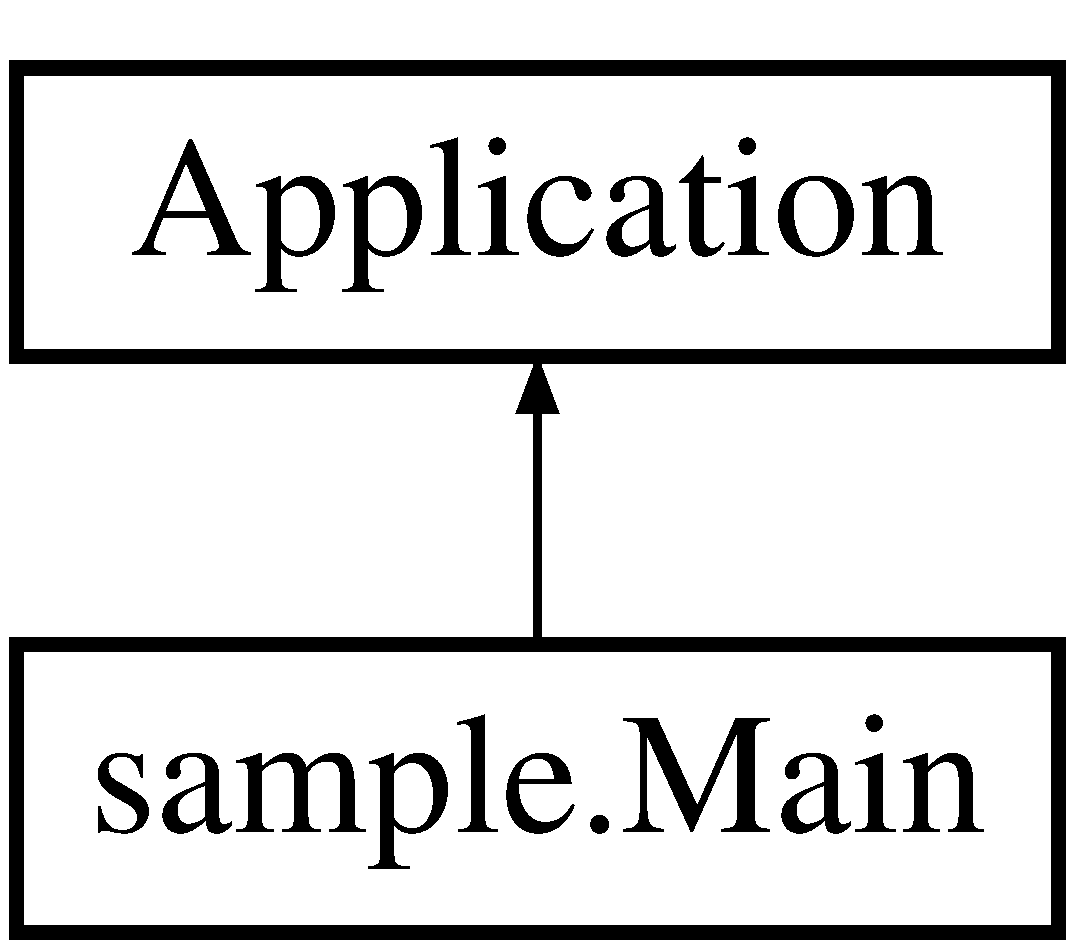
\includegraphics[height=2.000000cm]{classsample_1_1_main}
\end{center}
\end{figure}
\subsection*{Public Member Functions}
\begin{DoxyCompactItemize}
\item 
void \mbox{\hyperlink{classsample_1_1_main_a64ba37c898ca967654307543954cd09d}{start}} (Stage primary\+Stage)  throws Exception
\end{DoxyCompactItemize}
\subsection*{Static Public Member Functions}
\begin{DoxyCompactItemize}
\item 
static void \mbox{\hyperlink{classsample_1_1_main_ab70e98057c0f40b833a38ea10a74eceb}{main}} (String\mbox{[}$\,$\mbox{]} args)
\end{DoxyCompactItemize}


\subsection{Member Function Documentation}
\mbox{\Hypertarget{classsample_1_1_main_ab70e98057c0f40b833a38ea10a74eceb}\label{classsample_1_1_main_ab70e98057c0f40b833a38ea10a74eceb}} 
\index{sample\+::\+Main@{sample\+::\+Main}!main@{main}}
\index{main@{main}!sample\+::\+Main@{sample\+::\+Main}}
\subsubsection{\texorpdfstring{main()}{main()}}
{\footnotesize\ttfamily static void sample.\+Main.\+main (\begin{DoxyParamCaption}\item[{String \mbox{[}$\,$\mbox{]}}]{args }\end{DoxyParamCaption})\hspace{0.3cm}{\ttfamily [inline]}, {\ttfamily [static]}}

\mbox{\Hypertarget{classsample_1_1_main_a64ba37c898ca967654307543954cd09d}\label{classsample_1_1_main_a64ba37c898ca967654307543954cd09d}} 
\index{sample\+::\+Main@{sample\+::\+Main}!start@{start}}
\index{start@{start}!sample\+::\+Main@{sample\+::\+Main}}
\subsubsection{\texorpdfstring{start()}{start()}}
{\footnotesize\ttfamily void sample.\+Main.\+start (\begin{DoxyParamCaption}\item[{Stage}]{primary\+Stage }\end{DoxyParamCaption}) throws Exception\hspace{0.3cm}{\ttfamily [inline]}}



The documentation for this class was generated from the following file\+:\begin{DoxyCompactItemize}
\item 
src/sample/\mbox{\hyperlink{_main_8java}{Main.\+java}}\end{DoxyCompactItemize}

\chapter{File Documentation}
\hypertarget{_r_e_a_d_m_e_8md}{}\section{R\+E\+A\+D\+M\+E.\+md File Reference}
\label{_r_e_a_d_m_e_8md}\index{R\+E\+A\+D\+M\+E.\+md@{R\+E\+A\+D\+M\+E.\+md}}

\hypertarget{_alert_8java}{}\section{src/sample/\+Alert.java File Reference}
\label{_alert_8java}\index{src/sample/\+Alert.\+java@{src/sample/\+Alert.\+java}}
\subsection*{Classes}
\begin{DoxyCompactItemize}
\item 
class \mbox{\hyperlink{classsample_1_1_alert}{sample.\+Alert}}
\end{DoxyCompactItemize}
\subsection*{Packages}
\begin{DoxyCompactItemize}
\item 
package \mbox{\hyperlink{namespacesample}{sample}}
\end{DoxyCompactItemize}

\hypertarget{_color_square_8java}{}\section{src/sample/\+Color\+Square.java File Reference}
\label{_color_square_8java}\index{src/sample/\+Color\+Square.\+java@{src/sample/\+Color\+Square.\+java}}
\subsection*{Classes}
\begin{DoxyCompactItemize}
\item 
class \mbox{\hyperlink{classsample_1_1_color_square}{sample.\+Color\+Square}}
\end{DoxyCompactItemize}
\subsection*{Packages}
\begin{DoxyCompactItemize}
\item 
package \mbox{\hyperlink{namespacesample}{sample}}
\end{DoxyCompactItemize}

\hypertarget{_controller_8java}{}\section{src/sample/\+Controller.java File Reference}
\label{_controller_8java}\index{src/sample/\+Controller.\+java@{src/sample/\+Controller.\+java}}
\subsection*{Classes}
\begin{DoxyCompactItemize}
\item 
class \mbox{\hyperlink{classsample_1_1_controller}{sample.\+Controller}}
\end{DoxyCompactItemize}
\subsection*{Packages}
\begin{DoxyCompactItemize}
\item 
package \mbox{\hyperlink{namespacesample}{sample}}
\end{DoxyCompactItemize}

\hypertarget{_main_8java}{}\section{src/sample/\+Main.java File Reference}
\label{_main_8java}\index{src/sample/\+Main.\+java@{src/sample/\+Main.\+java}}
\subsection*{Classes}
\begin{DoxyCompactItemize}
\item 
class \mbox{\hyperlink{classsample_1_1_main}{sample.\+Main}}
\end{DoxyCompactItemize}
\subsection*{Packages}
\begin{DoxyCompactItemize}
\item 
package \mbox{\hyperlink{namespacesample}{sample}}
\end{DoxyCompactItemize}

%--- End generated contents ---

% Index
\backmatter
\newpage
\phantomsection
\clearemptydoublepage
\addcontentsline{toc}{chapter}{Index}
\printindex

\end{document}
